\chapter{Outras informações}

Considere um circuito lógico presente em um sistema de segurança de um cofre privado.
\begin{quote}
	Se a senha primaria estiver correta E (a leitura de digitais apresentar valor válido OU
	a leitura de íris apresentar valor válido),
	deve ser acendido um led azul, liberando o acesso.
	Caso contrário, deve ser acendido um led laranja.
\end{quote}

Expressão lógica:
$S.(D+I)$
em que S representa \textit{se a senha primaria estiver correta}, D
 \textit{se a leitura de digitais apresentar valor válido} e I \textit{se a leitura de íris apresentar valor válido}.

 \begin{table}[h]
 	\centering
 	\caption{Tabela verdade da expressão lógica}\label{table:tabelaVerdadeOutro}
 	\begin{tabular}{c|c|c|c}
 	%\hline
 		\textbf{S} & \textbf{D} & \textbf{I} & \textbf{S.(D+I)} \\
 		\hline
 		0 & 0 & 0 & 0\\\hline
 		0 & 0 & 1 & 0\\\hline
 		0 & 1 & 0 & 0\\\hline
 		0 & 1 & 1 & 0\\\hline
 		1 & 0 & 0 & 0\\\hline
 		1 & 0 & 1 & 1\\\hline
 		1 & 1 & 0 & 1\\\hline
 		1 & 1 & 1 & 1
 	\end{tabular}
 \end{table}

 \begin{figure}[htb]
	 \centering
	 \caption{\label{fig:desenhoOutro}Desenho do circuito}
	 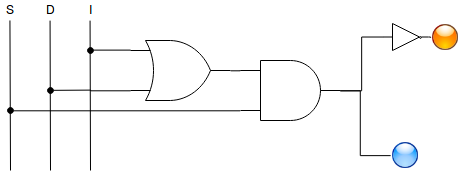
\includegraphics{img/desenhoOutro}
 \end{figure}
